\begin{frame}\begin{center}
\LARGE\textbf{Setup}
\end{center}\end{frame}
%-------------------------------------------------------------------------------
%-------------------------------------------------------------------------------
\begin{frame}\textbf{The Generalized Roy Model}
\begin{align*}\begin{array}{l@{\qquad}l}
\text{Potential Outcomes} &\text{Observed Outcome}\\
Y_1 = \mu_1(X) + U_1      &  Y = D Y_1 + (1 - D)Y_0 \\
Y_0 = \mu_0(X) + U_0      &\\
    & \\
\text{Choice} & \\
D = \mathrm{I}[\mu_D(X, Z) - V > 0] & \\
\end{array}
\end{align*}
\end{frame}

%-------------------------------------------------------------------------------
%-------------------------------------------------------------------------------
\begin{frame}\textbf{Treatment Status}

\begin{align*}
D &\qquad \text{self-selected} \\
\xi &\qquad \text{assigned} \\
A &\qquad  \text{actual}
\end{align*}
\end{frame}
%-------------------------------------------------------------------------------
%-------------------------------------------------------------------------------
\begin{frame}\textbf{Key Identifying Assumptions}
\begin{align*}
(Y_1, Y_0) & \indep D \\
(Y_1, Y_0) & \indep \xi \\
(Y_1, Y_0) & \indep A
\end{align*}

When do we have to worry about compliance?

\end{frame}
%-------------------------------------------------------------------------------
%-------------------------------------------------------------------------------
\begin{frame}
\begin{align*}
& E(Y\mid A = 1) - E(Y\mid A = 0) \\
& \qquad\qquad = E(Y_1\mid A = 1) - E(Y_0\mid A = 0)  \tag{by full compliance} \\
& \qquad\qquad = E(Y_1) - E(Y_0)  \tag{by randomization} \\
& \qquad\qquad = ATE = TT = TUT
\end{align*}
\end{frame}
%-------------------------------------------------------------------------------
%-------------------------------------------------------------------------------
\begin{frame}
What if we can only deny program participation to individuals who are willing to participate?
\begin{align*}
& E(Y\mid D= 1, A = 1) - E(Y\mid D = 1, A = 0) \\
& \qquad\qquad = E(Y_1\mid D= 1, A = 1) - E(Y_0\mid D=1, A = 0) \\
& \qquad\qquad = E(Y_1\mid D = 1) - E(Y_0 \mid D = 1)  \\
& \qquad\qquad = TT \neq ATE \neq TUT
\end{align*}
\end{frame}
%-------------------------------------------------------------------------------
%-------------------------------------------------------------------------------
\begin{frame}\textbf{Issues}\vspace{0.3cm}

\begin{itemize}\setlength\itemsep{0.5em}
\item Compliance
\item Imperfect Randomization
\item Ethical Concerns
\item Feasibility
\item Expenses
\item External Validity
\end{itemize}
\end{frame}
%-------------------------------------------------------------------------------
%-------------------------------------------------------------------------------
\begin{frame}\textbf{Challenges to Scaling Experiments}\vspace{0.3cm}

\begin{itemize}\setlength\itemsep{0.5em}
\item market equilibrium effects
\item spillovers
\item political reactions
\item context dependence
\item randomization or site-selection bias
\item piloting bias\vspace{0.3cm}
\end{itemize}

See \citet{Banerjee.2017} for a discussion of these challenges and their attempts to address them in their work.
\end{frame}
%-------------------------------------------------------------------------------
%-------------------------------------------------------------------------------
\begin{frame}\textbf{The Abdul Latif Jameel Poverty Action Lab}\vspace{0.3cm}

\begin{quote} The Abdul Latif Jameel Poverty Action Lab (J-PAL) is a network of 158 affiliated professors from 51 universities. Our mission is to reduce poverty by ensuring that policy is informed by scientific evidence. We do this through research, policy outreach, and training across six regional offices worldwide.\\\vspace{0.3cm}
\end{quote}


See their \href{https://www.povertyactionlab.org}{website} for an impressive amount of resources for running experiments.
\end{frame}
%-------------------------------------------------------------------------------
%-------------------------------------------------------------------------------
\begin{frame}
\begin{figure}
\caption{Book Recommendations}
\centering
	\subfloat[]{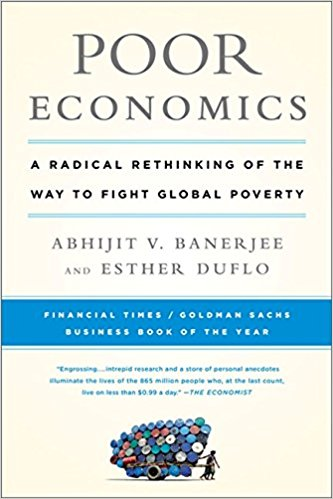
\includegraphics[width=0.40\linewidth]{fig-poor-economics}} \hspace{25pt}
	\subfloat[]{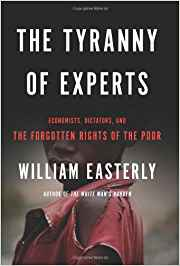
\includegraphics[width=0.40\linewidth]{fig-tyranny}}
\end{figure}
\end{frame}
%-------------------------------------------------------------------------------
%-------------------------------------------------------------------------------
